\chapter{Datasets}
\label{chap:datasets} 

This appendix contains visualisations of the annotation for each dataset, as well as some representative images. The charts show a breakdown of: (a) categories of annotation derived from corrections applied, (b) types of user actions and (c) annotation rate in annotations per minute. All three charts use a gaussian density estimate with $\sigma=\SI{5}{\minute}$. 

The \emph{penguin survey} charts are split into three parts (each part was annotated separately).

\newpage
\section{penguins}
\label{sec:penguins_details}

\begin{figure}[!h]
\centering
  \includegraphics[width=0.475\linewidth]{figures/annotation/screenshots/penguins.png}
  \hfill
  \includegraphics[width=0.475\linewidth]{figures/annotation/screenshots/penguins2.png}

\caption{Example images from the \emph{penguins} dataset, \cite{PenguinData}}
\label{fig:penguin_dataset}
\end{figure}

\begin{figure}[!h]
\centering
\includegraphics[width=1.0\linewidth]{charts/action_annotations/penguins.pdf}
\caption{Correction and detection types (top), user actions (middle), and annotation rate (bottom) for \emph{penguins} dataset.}
\label{fig:penguin_annotation}
\end{figure}



\pagebreak
\section{\texorpdfstring{$\mathrm{apples^1}$}{}}
\label{sec:apples1_details}

\begin{figure}[!h]
  \includegraphics[width=0.475\linewidth]{figures/annotation/screenshots/apples_big.png}
  \hfill
  \includegraphics[width=0.45\linewidth]{figures/annotation/screenshots/apples_small.png}
\caption{Example images from the $apples^1$ dataset.}
\label{fig:apples1_dataset}  
\end{figure}

\begin{figure}[!h]
\centering
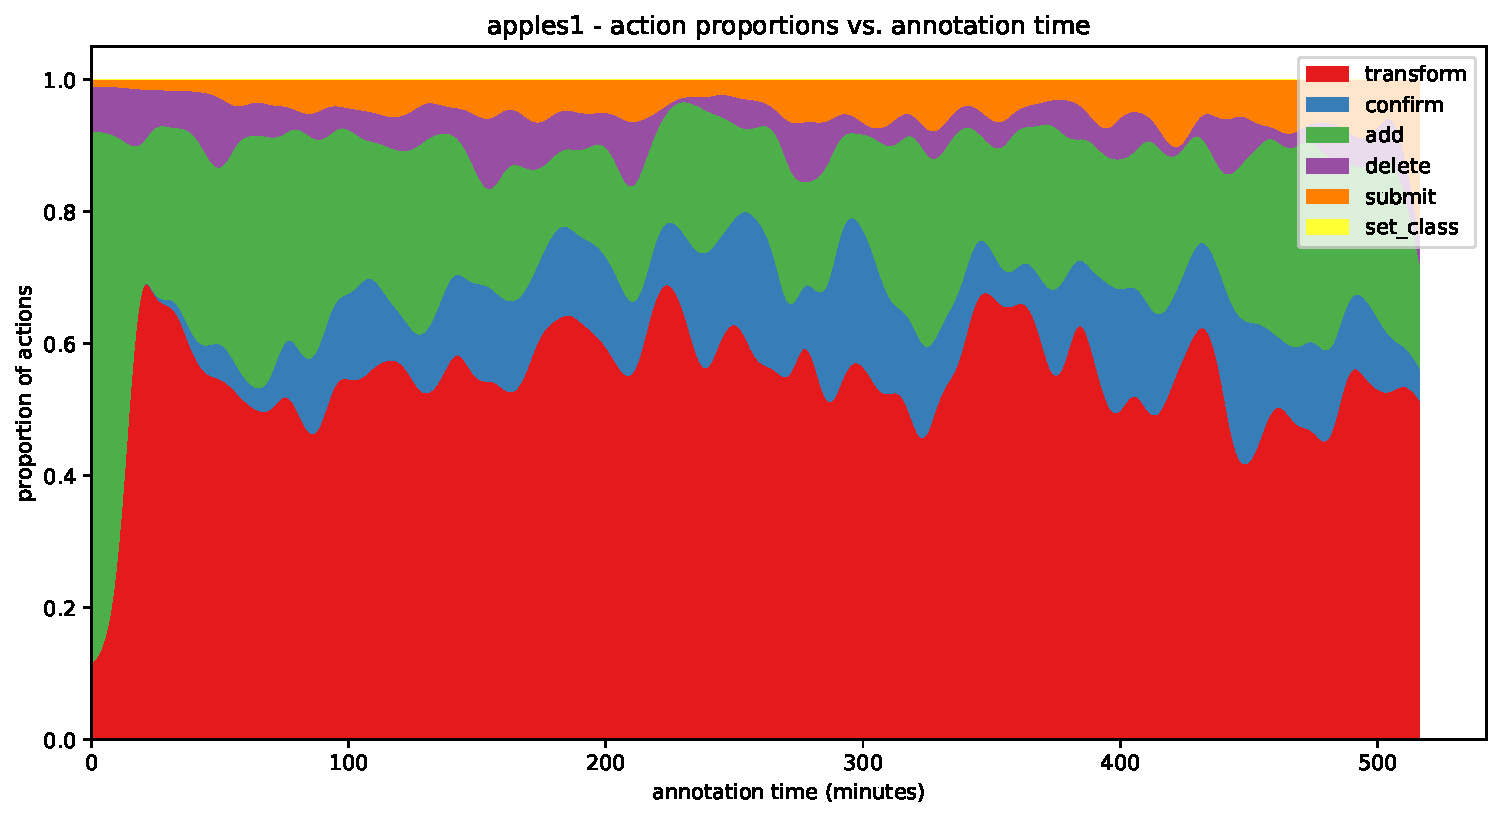
\includegraphics[width=1.0\linewidth]{charts/action_annotations/apples1.pdf}
\caption{Correction and detection types (top), user actions (middle), and annotation rate (bottom) for $apples^1$ dataset.}
\label{fig:apples1_annotation}
\end{figure}

\pagebreak
\section{\texorpdfstring{$\mathrm{apples^2}$}{}}
\label{sec:apples2_details}


\begin{figure}[!h]
  \includegraphics[width=0.475\linewidth]{figures/annotation/screenshots/apples2.png}
  \hfill
  \includegraphics[width=0.475\linewidth]{figures/annotation/screenshots/apples2_dark.png}
\caption{Example images from the $apples^2$ dataset.}
\label{fig:apples2_dataset}  
\end{figure}

\begin{figure}[!h]
\centering
\includegraphics[width=1.0\linewidth]{charts/action_annotations/apples2.pdf}
\caption{Correction and detection types (top), user actions (middle), and annotation rate (bottom) for $apples^2$ dataset.}
\label{fig:apples2_annotation}
\end{figure}

\pagebreak
\section{buoys}
\label{sec:buoys_details}


\begin{figure}[H]
  \includegraphics[width=0.475\textwidth]{figures/annotation/screenshots/buoys.png}
  \hfill
  \includegraphics[width=0.475\textwidth]{figures/annotation/screenshots/buoys2.png}
  \caption{Example images from the \emph{buoys} dataset of mussel farm buoys captured from a camera attached to another buoy }
  \label{fig:buoys_dataset}
\end{figure}

\begin{figure}[!h]
\centering
\includegraphics[width=1.0\linewidth]{charts/action_annotations/buoys.pdf}
\caption{Correction and detection types (top), user actions (middle), and annotation rate (bottom) for $buoys_d$ dataset.}
\label{fig:buoys_annotation}
\end{figure}

\pagebreak
\section{fisheye}
\label{sec:fisheye_details}


\begin{figure}[H]
\begin{center}
  \includegraphics[width=0.5\textwidth]{figures/annotation/screenshots/victor.png}
\end{center}
  \caption{Example image from the \emph{fisheye} dataset of fish-eye lens head and cellphone detection }
\end{figure}

\begin{figure}[!h]
\centering
\includegraphics[width=1.0\linewidth]{charts/action_annotations/fisheye.pdf}
\caption{Correction and detection types (top), user actions (middle), and annotation rate (bottom) for $fisheye$ dataset.}
\label{fig:fisheye_annotation}
\end{figure}


\pagebreak
\section{branches}
\label{sec:branches_details}


\begin{figure}[!h]
  \includegraphics[width=0.475\textwidth]{figures/annotation/screenshots/branches3.png}
  \includegraphics[width=0.475\textwidth]{figures/annotation/screenshots/branches2.png}  
  
  \caption{Example images from \emph{branches}, tree branch intersection detection}
\end{figure}

\begin{figure}[!h]
\centering
\includegraphics[width=1.0\linewidth]{charts/action_annotations/branches.pdf}
\caption{Correction and detection types (top), user actions (middle), and annotation rate (bottom) for $branches$ dataset.}
\label{fig:branches_annotation}
\end{figure}

\pagebreak
\section {scallops}
\label{sec:scallop_details}


\begin{figure}[!h]
  \includegraphics[width=0.475\linewidth]{figures/annotation/screenshots/scallops.png}
  \hfill
  \includegraphics[width=0.475\linewidth]{figures/annotation/screenshots/scallops3.png}
\caption{Example images from the \emph{scallop} dataset.}
\label{fig:scallop_dataset}  
\end{figure}

\begin{figure}[!h]
\centering
\includegraphics[width=1.0\linewidth]{charts/action_annotations/scallops.pdf}
\caption{Correction and detection types (top), user actions (middle), and annotation rate (bottom) for $scallops_e$ dataset.}
\label{fig:scallop_annotation}
\end{figure}

\pagebreak
\section {penguin survey}
\label{sec:penguin_survey_details}


\begin{figure}[!h]
\centering
  \includegraphics[width=0.475\linewidth]{figures/annotation/screenshots/penguins_aerial.png}
  \hfill
  \includegraphics[width=0.475\linewidth]{figures/annotation/screenshots/penguins_aerial2.png}
  \caption{}
\caption{ Example images from the \emph{penguin survey} dataset.}
\label {fig:penguin_aerial_examples}
\end{figure}

\begin{figure}[!h]
\centering
\includegraphics[width=1.0\linewidth]{charts/aerial_penguins/action_annotations/cotter_a.pdf}
\caption{Correction and detection types (top), user actions (middle), and annotation rate (bottom) for $cotter$ subset of the $penguin\:survey$ dataset.}
\label{fig:cotter_annotation}
\end{figure}

\pagebreak
\begin{figure}[H]
\begin{minipage}[c][\textheight]{\textwidth}
\centering
\includegraphics[width=1.0\linewidth]{charts/aerial_penguins/action_annotations/hallett_a.pdf}
\includegraphics[width=1.0\linewidth]{charts/aerial_penguins/action_annotations/royds_a.pdf}
\caption{  Correction and detection types (top), user actions (middle), and annotation rate (bottom) for the $hallett$ (top), $royds$ (bottom) subsets of the $penguin\:survey$ dataset }
\label{fig:royds_annotation}
\end{minipage}
\end{figure}


\pagebreak
\section {seals}
\label{sec:seals_details}


\begin{figure}[!h]
\centering
  \includegraphics[width=0.475\linewidth]{figures/annotation/screenshots/seals_small2.png}
  \hfill
  \includegraphics[width=0.45\linewidth]{figures/annotation/screenshots/seals_big.png}
  \caption{}
\caption{ Example images from the \emph{seals} dataset.}
\label {fig:seals_examples}
\end{figure}

\begin{figure}[!h]
\centering
\includegraphics[width=1.0\linewidth]{charts/action_annotations/seals1.pdf}
\caption{ Correction and detection types (top), user actions (middle), and annotation rate (bottom) for $seals$ dataset }
\label{fig:seals_annotation}
\end{figure}

\pagebreak
\section {\texorpdfstring{$\mathrm{seals_b}$}{}}
\label{sec:seals2_details}

\begin{figure}[!h]
\centering
\includegraphics[width=1.0\linewidth]{charts/action_annotations/seals2.pdf}
\caption{ Correction and detection types (top), user actions (middle), and annotation rate (bottom) for $seals_b$ dataset }
\label{fig:seals2_annotation}
\end{figure}

\pagebreak
\section {scott base}
\label{sec:scott_base_details}


\begin{figure}[!h]
\centering
  \includegraphics[width=0.475\linewidth]{figures/annotation/screenshots/scott_base_storm.png}
  \hfill
  \includegraphics[width=0.45\linewidth]{figures/annotation/screenshots/scott_base_sunny.png}
  \caption{}
\caption{ Example images from the \emph{scott base} dataset.}
\label {fig:scott_base_examples}
\end{figure}

\begin{figure}[!h]
\centering
\includegraphics[width=1.0\linewidth]{charts/action_annotations/scott_base.pdf}
\caption{ Correction and detection types (top), user actions (middle), and annotation rate (bottom) for $scott\:base$ dataset }
\label{fig:scott_base_annotation}
\end{figure}

\chapter{Source code and datasets}
\label{chap:resources} 

The source code to both parts of the \gls{VBA} annotation tool are open source, the source code is in two parts: 

\begin{itemize}
    \item \href{http://www.github.com/saulzar/detection}{Object detection trainer} 
    \item \href{http://www.github.com/saulzar/annotate}{Server and web annotation client}
\end{itemize}
 
  
Datasets are published in two parts:
 
 \begin{itemize}
\item \href{http://academictorrents.com/details/d8ceccf6d9a57b799003205e0567e630b0ecb90e}{Segmentation dataset \emph{trees}} \par
A collection of images annotated with segmentation masks from the study in Chapter~\ref{chap:bootstrap}.

\item \href{http://academictorrents.com/details/e780e1a9e898e53e72c16cb5fcc6d61d90cc4d27}{Annotated object detection datasets} \par
The full set of ten annotated object detection datasets from Chapter~\ref{chap:annotation}. All with annotations, raw training and annotation logs, trained models (run-able using the object detection trainer above), most with images (\emph{branches}, $apples^1$, $apples^2$, \emph{penguins}, \emph{buoys}, \emph{scallops}).

\end{itemize}

\chapter{MEGM gradient}
\label{chap:megm_appendix} 

The gradient for the \gls{MEGM} loss function as used in Chapter~\ref{chap:bootstrap} for metric learning. I adjusted the \gls{NCA} derivative found in \cite {Salakhutdinov2007a} to give the derivative for \gls{MEGM} output for the $ i^{th} $ training case and $ t^th $ class:

\begin{multline}
\label{eq:megm_grad}
\frac{\partial \mathcal{E}_{megm}}{\partial f(x_{ti})} = 
  -2 \bigg( \sum_{j:c_i = c_j}  m_{ti} {p_{ij} \Big( d_{ij} - \sum_z{p_{iz}d_{iz}} \Big) } \bigg)\\
  +2 \bigg( \sum_{j:c_i = c_j} m_{tj}{p_{ji}d_{ji} - \sum_z{\Big( \sum_{q:c_z = c_q}{p_{zq}} \Big) m_{tz}p_{zi}d_{zi}   }} \bigg)
\end{multline}

Where $ err_{ti} $ is shorthand for the partial derivative $ \hat{y_{ti}} $ with respect to \gls{MSE}, and $ d_{ij} = f(x_i) - f(x_j) $ is shorthand for the difference between the descriptor vectors. The formula differs from the \gls{NCA} derivative only by the $ err_{ti} $ term.

\begin{equation}
m_{ti} = \frac{\partial \mathcal{E}_{megm}}{\partial \hat{y_{ti}}} = -2 (y_{ti} - \hat{y_{ti}})
\label{eq:megm_partial}
\end{equation}